% !TEX root = ../lectures.tex
\section{From Linear to Non-Linear: The Formation of Shock Waves}

This section aims to qualitatively illustrate how the formation of shock waves is a natural and, consequently, a frequent phenomenon in astrophysical environments.

In the linear regime, small perturbations in a medium propagate at the sound speed, \( c_{s,0} \), which we earlier defined in terms of the pressure \( P_0 \) and density \( \rho_0 \) of the medium (see eq.~\ref{eq:cs02}). For linear waves, \( c_{s,0} \) is assumed to be constant across the medium. 

When the amplitude of the perturbation increases, the wave enters the non-linear regime, where the propagation speed depends on the local density. Specifically:  
\[
c_s^2 \propto \frac{P}{\rho} \propto \rho^{\gamma - 1},
\]  
where \( \gamma \sim 5/3 \) is the adiabatic index of the medium. High-density regions propagate faster than low-density regions. This effect fundamentally alters the wave's behavior.  

Imagine a sinusoidal wave (as the solution found in eq.~\ref{eq:rhowaveform}) traveling through a medium. As density peaks (crests) move faster than the troughs, the waveform becomes increasingly asymmetric. Over time, this leads to the steepening of the wave front until the crest overtakes the trailing edge. At this point, the wave profile develops a physical inconsistency --- a \emph{multi-valued} solution (see fig.~\ref{fig:landau}). The resolution to this breakdown is the formation of a \emph{shock wave}, a discontinuity in the fluid properties.

As a direct consequence of their formation process, shock waves exhibit several distinctive properties:
%
\begin{itemize}
\item Shock waves are associated with matter moving at speeds exceeding the local sound speed. This supersonic motion compresses and heats the medium, creating a steep discontinuity.  
\item The medium cannot adjust to changes induced by the shock wave fast enough. As a result, fluid variables such as density, temperature, and velocity undergo abrupt \emph{jumps} at the shock front.  
\item The shock propagates faster than any signal can travel within the medium. Consequently, regions ahead of the shock (pre-shock) remain unaware of the disturbance until the shock front reaches them.  
\end{itemize}

\begin{figure}[!t]
\centering
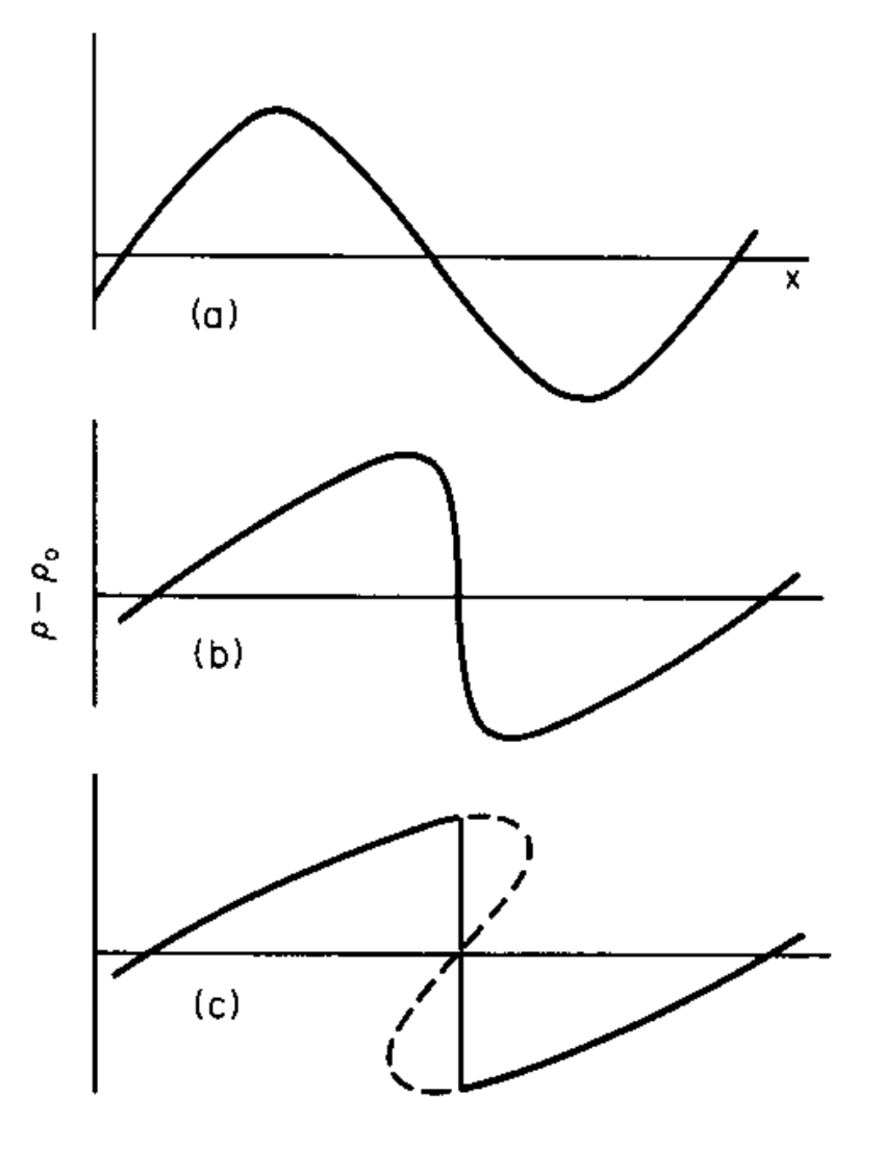
\includegraphics[width=0.5\textwidth]{figures/shocklandau.pdf}
\caption{}
\label{fig:landau}
\end{figure}

In fact, shock waves are a ubiquitous feature in astrophysical environments, reflecting the variety of processes that drive supersonic motion. 
%
Notable examples include:
\begin{itemize}
\item Fast stellar winds collide with the interstellar medium, forming bow shocks or termination shocks.  
\item Supernova blast waves plow into the surrounding medium.  
\item In gamma-ray bursts, colliding relativistic shells generate shocks within the ejecta.  
\item Matter falling onto compact objects like neutron stars or black holes forms accretion shocks.  
\item Shock waves develop as material accretes onto galaxy clusters' hydrostatic intracluster medium.  
\end{itemize}

Their presence in is a testament to the dynamic, high-energy processes shaping the universe.

\end{document}

\section{Interstellar Shock Waves}

\begin{figure}[!t]
\centering
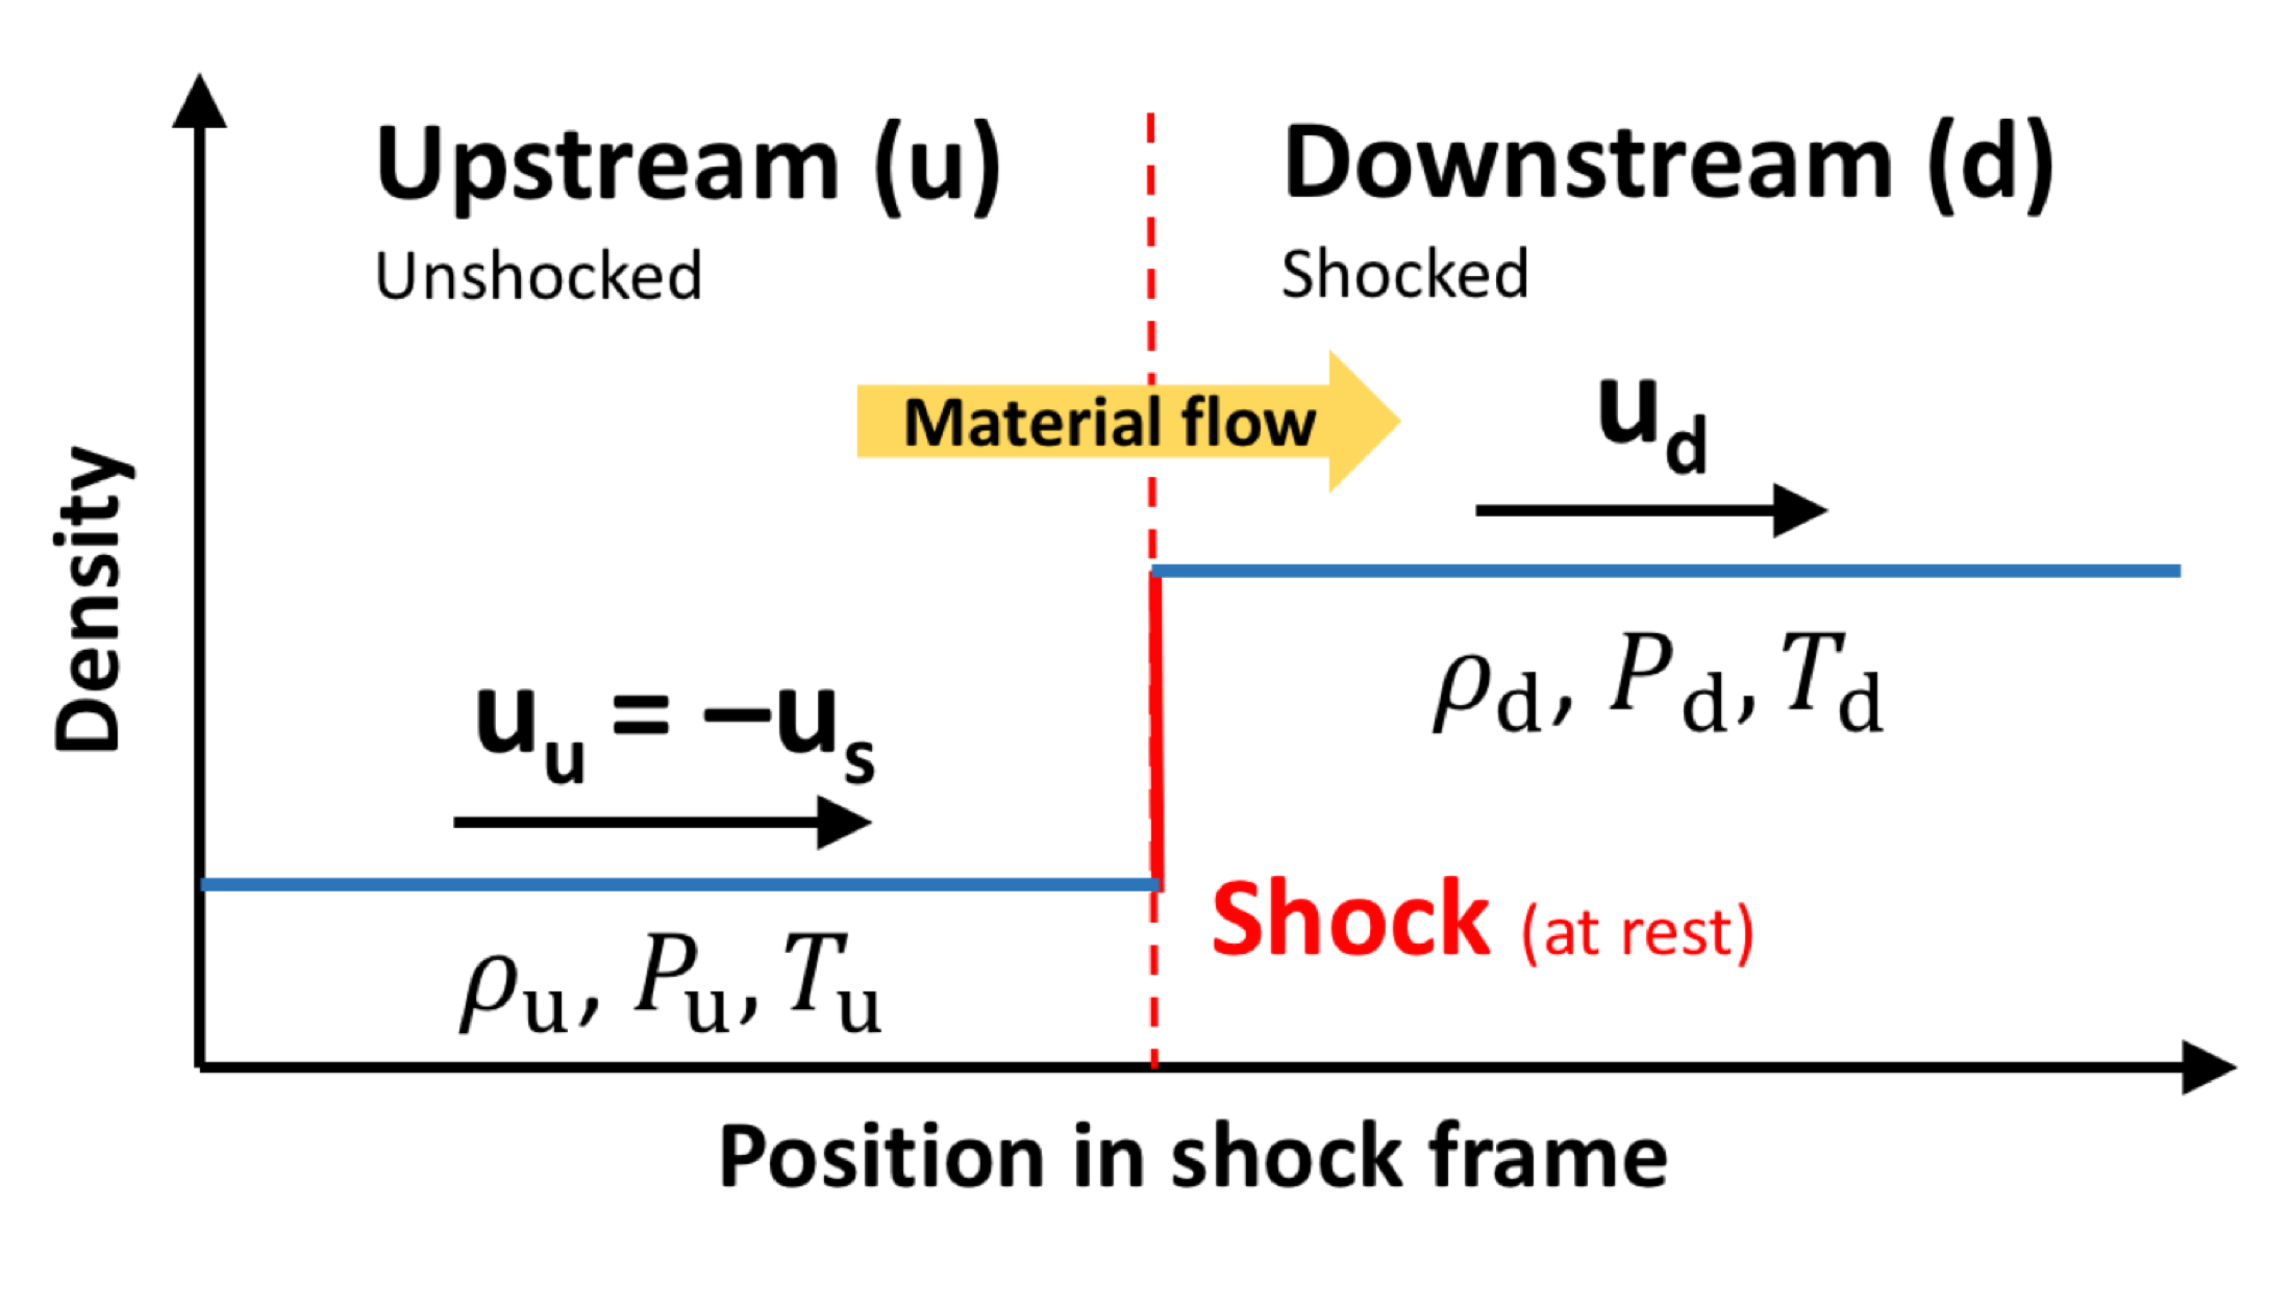
\includegraphics[width=0.5\textwidth]{figures/downupstream.pdf}
\caption{}
\end{figure}

Hydrodynamics often presents discontinuous solutions, meaning that there exist surfaces where physical quantities change abruptly. Mathematically, this is represented by differing values at the left and right limits of a point. However, physically, this discontinuity is not infinitely sharp as suggested in mathematical theory; rather, the change occurs over a region smaller than all other physical scales involved. 
%
A \emph{shock} is a specific type of discontinuity characterized by a surface that separates two fluid regions with differing properties. Importantly, this surface allows for the transfer of mass, momentum, and energy across it.

As seen beforehand, shocks are a natural consequence in the non-linear regime of fluid dynamics or magnetohydrodynamics (MHD).

Shocks are especially relevant in astrophysics; the gas post-shock emits significantly more than pre-shock gas, making these events more detectable.

Unlike terrestrial shocks, astrophysical shock waves are predominantly \textbf{collisionless}. 
%
In standard atmospheric conditions, where the number density of particles is approximately \( n \sim 10^{23} \, \text{cm}^{-3} \), and the cross-section for collisions\footnote{In the case of neutral particles, the hard sphere approximation holds true, where \( \sigma = \pi (r_A + r_B)^2 \) with \( r \) denoting the atomic radii of the colliding atoms.} around \( \sigma \sim 10^{-16}~\text{cm}^2 \), the mean free path \( \lambda \simeq 1 / (n \sigma) \) of a particle is \( \simeq 10^{-7}~\text{cm} \). 
%
In such conditions, \textbf{collisions} between particles are frequent, leading to the transformation of ordered kinetic energy into disordered (thermal) kinetic energy, characteristic of a collisional shock.

In contrast, astrophysical environments, where most particles are ionized, present a different scenario. The cross-sections for ionized particles are typically on the order of \( \sigma \sim \pi r_0^2 \sim 10^{-26}~\text{cm}^2 \) as $r_0 \sim$~fm is now the \textbf{nuclear} radius.
%
More importantly, these environments have much lower particle densities, about \( n \sim 1~\text{cm}^{-3} \). As a result, the mean free path in such settings is \( \gg \) Mpc! 
%
This means that the formation of the shock and its energy dissipation mechanisms do not primarily occur through particle collisions or Coulomb interactions. Instead, these processes are predominantly governed by interactions with the ambient magnetic field. The detailed microphysics of astrophysical shocks are complex and beyond the scope of this discussion.

Despite the microscale complexity at discontinuities (e.g., finite conductivity determining the size), conservation laws of mass, momentum, and energy remain applicable.

For non-relativistic shock waves, we can define the reference frame of the unshocked medium or \textbf{Galaxy frame}, where \( u^\prime_1 = 0 \),
the shock propagates into the unshocked medium at a speed \( u^\prime_s \), while the speed of shocked gas is \( u^\prime_2 (< u^\prime_s) \).

More convenient is to use a frame of reference  where the discontinuity surface is stationary, with \( u_s = 0 \). So the upstream medium approaches it at a speed \( u_1 = -u^\prime_s \), while the shocked fluid moves away from the shock front at a speed \( u_2 = u^\prime_s - u^\prime_2 \).
%
Consequently, the relative speed between the shocked and unshocked fluids is \( u_{\text{rel}} = u_1 - u_2 \).

In the following, it will be easier to refer our equations to the \textbf{shock front frame}, and we will categorize the physical quantities based on their position relative to the shock: those \textbf{upstream} of the shock are labeled as '1' and those \textbf{downstream} as '2'.\footnote{Use instead u and d.}

In the context of shock dynamics, we will focus on key thermodynamic quantities: density, pressure, temperature, and momentum across the two media (upstream and downstream of the shock). To analyze these, we first want to write conservation equations in the form \( \frac{dJ}{dz} = 0 \), where \( J \) represents the flux of a conserved quantity (be it mass, energy, or momentum).

Following this approach, it implies:
%
\begin{equation}
\int_{-\epsilon}^{\epsilon} \frac{dJ}{dx} = J_2 - J_1 = 0
\end{equation}

As common here, we introduce the notation \( [J]_{\text{sh}} = 0\) to denote the change in the flux across the shock expressed as \( J_2 - J_1 = 0 \). 

Let us summarize the key transport equations for a fluid, assuming that the only acting force density is the pressure gradient \( \nabla P \), and neglecting the effects of magnetic or gravitational fields.

First, the mass continuity equation is given by:
%
\begin{equation}
\frac{\partial \rho}{\partial t} + \nabla \cdot (\rho \mathbf{u}) = 0
\end{equation}
%
where \( \rho \) represents the fluid density, and \( \mathbf{u} \) is the fluid velocity.

Next, the conservation of momentum per unit volume is described by:
%
\begin{equation}
\rho \frac{\partial \mathbf{u}}{\partial t} + \rho (\mathbf{u} \cdot \nabla) \mathbf{u} = -\nabla P
\end{equation}

Finally, the conservation of energy per unit volume is expressed as:
%
\begin{equation}
\frac{\partial}{\partial t} \left( \frac{1}{2} \rho u^2 + \rho U \right) + \nabla \cdot \left[ \mathbf{u} \left( \frac{1}{2} \rho u^2 + \rho U + P \right) \right] = 0
\end{equation}
%
here \( \epsilon = \rho U \) denotes the internal energy per unit volume.

For our analysis, we focus on a one-dimensional (planar) shock in a stationary state (\( \partial_t \rightarrow 0 \)) and apply these conservation laws within the reference frame where the discontinuity is stationary.

Applying the mass continuity equation, we derive:
%
\begin{equation}\label{eq:mass}
\frac{\partial}{\partial z} (\rho u) = 0
\end{equation}

Next, from the momentum equation, and utilizing the mass continuity equation in Eq.~\ref{eq:mass}, we obtain:
%
\begin{equation}
\rho u \frac{\partial u}{\partial z} = -\frac{\partial P}{\partial z}  \, \rightarrow \, \frac{\partial}{\partial z} (P + \rho u^2) = 0 
\end{equation}

%Here, \( P_{\text{g}} \) represents the gas pressure.

Moving to the energy equation and again invoking the continuity equation, we find:
%
\begin{equation}
\frac{\partial}{\partial z} \left( \rho u \left[ \frac{1}{2} u^2 + U + \frac{P}{\rho} \right] \right) = 0 
\end{equation}

This can be expressed in terms of specific enthalpy \( w \) (see Appendix):
%
\begin{equation}
w = U + \frac{P}{\rho} = \frac{\gamma}{\gamma - 1}\frac{P}{\rho}
\end{equation}

Therefore, we arrive at the equation:
%
\begin{equation}
\frac{\partial}{\partial z} \left( \frac{1}{2} u^2 + \frac{\gamma}{\gamma - 1}\frac{P}{\rho} \right) = 0 
\end{equation}

Summarizing, assuming planar geometry, and in the frame of the shock, the conservation of fluxes of mass, momentum energy across the shock write
%
\begin{remark}
\begin{eqnarray}
\left[ \rho u \right]_{\rm sh} & = & 0 \label{eq:RH1} \\
\left[ \rho u^2 + P \right]_{\rm sh} & = & 0 \label{eq:RH2} \\
\left[ \frac{1}{2} u^2 +\frac{\gamma}{\gamma - 1} \frac{P}{\rho} \right]_{\rm sh} & = & 0 \label{eq:RH3}
\end{eqnarray}
\end{remark}

These conditions are known as the \textbf{Rankine-Hugoniot jump conditions}. They represent the dynamical equations for solutions that express conservation across the discontinuity of a shock, essentially establishing relationships between quantities on either side of the shock front.

We are dealing with three unknowns and have three corresponding equations. Apart from the trivial solution where all quantities remain constant, our aim is to derive the non-trivial solution.

To proceed, we remind the definition of sound speed:
%
\begin{equation}
c_{\text{s}} = \left( \frac{\partial P}{\partial \rho} \right)^{1/2} = \left(\frac{\gamma P}{\rho}\right)^{1/2}
\end{equation}

Here, we assume an ideal gas so the equation of state is \( P = K \rho^\gamma \), with \( \gamma \) being the ratio of specific heats. For a mono-atomic gas, in particular, \( \gamma = 5/3 \).

We then define the Mach number as the ratio of the shock speed to the sound speed in region \( i \), denoted as \( \mathcal{M}_i = v_i / c_{\text{s}} \). From this, it follows that:
%
\begin{equation}
\rho_i u_i^2 + P_i = \rho_i c_{\text{s}, i}^2 \left( \frac{u_i^2}{c_{\text{s},i}^2} \right) + P_i = (1 + \gamma \mathcal{M}_i^2) P_i
\end{equation}

If we fix the quantities in the upstream region,  $\rho_1$,  $u_1$ and $P_1$, hence solving the equations for the downstream using Eq.s~\ref{eq:RH1}-\ref{eq:RH3} will lead us to (see Appendix):
%
\begin{eqnarray}
\frac{\rho_2}{\rho_1} & = & \frac{u_1}{u_2}=\frac{(\gamma +1) \mathcal M_1^2}{(\gamma - 1) \mathcal M_1^2+2} \\
\frac{P_2}{P_1} & = & \frac{2\gamma \mathcal M_1^2}{\gamma +1}-\frac{\gamma -1}{\gamma +1} \\
\frac{T_2}{T_1} & = & \frac{\left[2\gamma \mathcal M_1^2 -(\gamma - 1) \right] \left[ (\gamma - 1) \mathcal M_1^2 + 2 \right]}{(\gamma + 1)^2 \mathcal M_1^2}
\end{eqnarray}

Under the assumption of strong shock conditions, characterized by \( \mathcal{M}_1 \gg 1 \), and considering a monoatomic gas with \( \gamma = 5/3 \), we can deduce the jump in density:
%
\begin{remark}
\begin{equation}
r = \frac{\rho_2}{\rho_1} = \frac{u_1}{u_2} = \frac{\gamma + 1}{\gamma - 1} = 4
\end{equation}
\end{remark}
%
here, \( r \) represents the compression factor, defined as \( \frac{\rho_2}{\rho_1} \). This factor is dependent on the adiabatic index \( \gamma \) and the Mach number of the shock. It's noteworthy that the compression factor cannot exceed 4.

For the pressure jump, we obtain:
%
\begin{equation}
\frac{P_2}{P_1} = \frac{2 \gamma}{\gamma + 1} \mathcal{M}_1^2 = \frac{5}{4} \mathcal{M}_1^2 
\end{equation}

From the frame of reference at the discontinuity, we observe an approaching gas with velocity \( u_1 \), which is altered to \( u_2 \approx \frac{1}{4}u_1 \) on the opposite side. Consequently, the plasma is decelerated and becomes denser.
%
However, energy conservation dictates that this energy must transform into \textbf{heat}. Examining the temperature ratio \( \frac{T_2}{T_1} \) under the same conditions, we find:
%
\begin{equation}
\frac{T_2}{T_1} = \frac{2 \gamma (\gamma - 1)}{(\gamma +1)^2} \mathcal{M}_1^2
\end{equation}

Therefore:
%
\begin{remark}
\begin{equation}
k_B T_2 = k_B T_1 \frac{2 \gamma (\gamma - 1)}{(\gamma +1)^2} \frac{u_1^2}{c_{\text{s},1}^2} = \frac{3}{16} m_p u_1^2
\end{equation}
\end{remark}

In this equation, we have utilized \( \rho_i = n_i m_p \), \( \mathcal{M}_i^2 = \frac{u_i^2}{c_{\text{s},i}^2} \), \( c_{\text{s},i}^2 = \frac{\gamma P_i}{\rho_i} \), and \( P_i = n_i k_B T_i \).

It's interesting to note that for typical astrophysical shocks, with \( u_1 \gtrsim 10^4 \) km/s, the temperature \( T_2 \) reaches approximately \( \sim 10^7 \) K.
%
This is what happens for example in a supernova explosion \( \mathcal M \sim 10^3 \) or in a GRB.  The plasma crosses shocks and heats up until it starts radiating in X-ray.

In summary, shocks convert \textbf{bulk kinetic energy of upstream medium to thermal (internal) energy downstream}.

\begin{remark}
The plasma behind the shock is
\begin{itemize}
\item Compressed \( \rho_2 = 4 \rho_1 \)
\item Slown down \( v_2 = \frac{1}{4} v_1 \)
\item Heated \( T_2 \ll T_1 \)
\end{itemize}
\end{remark}

The transformation of inflow kinetic energy into thermal energy in shock waves is accompanied by the generation of entropy. The key to this transformation is the collisions among particles within the shock wave. These collisions convert the ordered bulk kinetic energy, where particle velocities are aligned, into disordered internal kinetic energy, or heat.

However, as we have previously noted, the mean free path for collisions in astrophysical conditions can be macroscopically large. In such scenarios, energy exchange among particles is mediated by electromagnetic fields.
%
Therefore, the thickness of the shock is more characterized by the non-relativistic Larmor radius of a proton. This radius reflects the scale over which particles are deflected by the magnetic field present at the shock front.

Considering a typical proton velocity of \( \sim 10^4 \) km/s in a supernova explosion, and within a typical galactic magnetic field of \( 1 \mu \)G, the Larmor radius (\( r_{\text{B}} \)) is calculated as:
%
\begin{equation}
r_{\text{B}} = \frac{m_p v c}{e B} \simeq 10^{10}~\text{cm}
\end{equation}

When compared to typical lengths involved in supernova (SN) explosions, which are on the order of a parsec (see later), the shock thickness is several orders of magnitude smaller. Therefore, in the grand scale of such astrophysical phenomena, the approximation of an infinitely thin shock layer is justified.

Finally, we want to compute the post-shock Mach number \( M_2 \):
%
\begin{equation}
\mathcal M_2 = \frac{u_2}{c_{\rm s,2}} = \mathcal M_1 \frac{u_2}{u_1} \frac{c_1}{c_2} = \mathcal M_1 \frac{u_2}{u_1} \left( \frac{T_1}{T_2} \right)^{1/2}
\end{equation}
%
in the strong shock limit:
%
\begin{equation}
\mathcal M_2 = \mathcal M_1 \frac{\gamma - 1}{\gamma + 1} \left[ \frac{(\gamma + 1)^2}{2\gamma(\gamma - 1) \mathcal M_1^2} \right]^{1/2} = \left( \frac{\gamma - 1}{2\gamma} \right)^{1/2} \simeq 0.45 
\end{equation}
%
so a shock converts supersonic gas into subsonic gas.
%
In doing so, it increases the specific entropy of the gas by an amount~(see appendix):
%
\begin{equation}
s_2 - s_1 = c_{\rm P} \ln \left(\frac{T_2}{T_1}\right) - \frac{k}{m} \ln \left( \frac{P_2}{P_1} \right)
\end{equation}
%
In another terminology, a shock changes the entropy shifting gas to a higher adiabat.

Notice then that the non trivial solution makes sense only if the Mach number $M_1$ is larger than one. In the opposite case, we the variation of entropy would be in the sense to decrease it, which is not allowed by second principle of thermodynamics. 
%
In other words we would have invented a system to transform heat in ordered work! Shocks can only form in supersonic motion.

\subsection{Supernovae in the Milky Way}

Historical SNe: Kepler 1604, {\color{red}Tycho SNR 1572}, SN1006 SNR, Cas A 1680?

We distinguish between: 
%
\begin{itemize}
\item Core collapse supernovae (Type II, Ib/c,..)
\begin{itemize}
\item Progenitor: Massive star (\( \gtrsim 8~M_\odot \))
\item Energy source: gravitational collapse (\( \gtrsim 10^{53} \)~erg) 
\item Kinetic energy: \( \sim 10^{51} \)~erg
\item Ejecta mass \( >4~M_\odot \)  
\item Neutron star (or BH)
\end{itemize}
\item Thermonuclear supernovae (Type Ia)
\begin{itemize}
\item Progenitor: accreting CO white dwarf, or merging white dwarfs 
\item Energy source: nuclear fusion (C/O -> Fe-group)
\item Kinetic energy: \( 1.2 \times 10^{51} \) erg
\item Ejecta mass \( \sim 1.4~M_\odot \)
\item Total disruption of star
\end{itemize}
\end{itemize}